\documentclass[tikz,border=8pt]{standalone}
\usepackage{amsmath,amssymb}
\usepackage{tikz}
\usetikzlibrary{arrows.meta,calc,angles}

\begin{document}
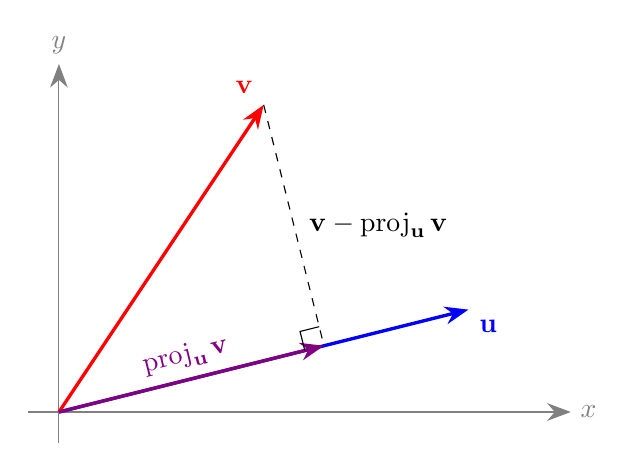
\begin{tikzpicture}[scale=1.3, >={Stealth[length=3mm]}]
  \draw[->, gray] (-0.3,0) -- (5,0) node[right] {$x$};
  \draw[->, gray] (0,-0.3) -- (0,3.4) node[above] {$y$};
  \coordinate (O) at (0,0);
  \coordinate (U) at (4,1);
  \coordinate (V) at (2,3);
  \coordinate (P) at ($(O)!(V)!(U)$);
  \draw[->, very thick, blue] (O) -- (U) node[below right] {$\mathbf{u}$};
  \draw[->, very thick, red]  (O) -- (V) node[above left] {$\mathbf{v}$};
  \draw[->, very thick, violet] (O) -- (P)
    node[midway, above, sloped] {$\operatorname{proj}_{\mathbf{u}}\mathbf{v}$};
  \draw[dashed] (V) -- (P);
  \pic[draw, angle radius=2.5mm] {right angle = V--P--O};
  \node[right=2pt] at ($(V)!0.5!(P)$) {$\mathbf{v}-\operatorname{proj}_{\mathbf{u}}\mathbf{v}$};
\end{tikzpicture}
\end{document}
